\documentclass[twoside,twocolumn]{article}
\usepackage[utf8]{inputenc}
\usepackage{hanging}
\usepackage[sc]{mathpazo}
\usepackage[T1]{fontenc} 
\linespread{1.05} 
\usepackage{microtype} 
\usepackage[english]{babel}
\usepackage[hmarginratio=1:1,top=28mm,columnsep=20pt]{geometry} 
\usepackage[hang, small,labelfont=bf,up,textfont=it,up]{caption} 
\usepackage{booktabs} 
\usepackage{lettrine}
\usepackage{graphicx} 
\usepackage{enumitem} 
\setlist[itemize]{noitemsep} 
\usepackage{abstract} 
\renewcommand{\abstractnamefont}{\normalfont\bfseries}
\renewcommand{\abstracttextfont}{\normalfont\small\itshape} 
\usepackage{titlesec}
\renewcommand\thesection{\Roman{section}} 
\renewcommand\thesubsection{\roman{subsection}} 
\titleformat{\section}[block]{\large\scshape\centering}{\thesection.}{1em}{}
\titleformat{\subsection}[block]{\large}{\thesubsection.}{1em}{} 
\usepackage{fancyhdr} 
\pagestyle{fancy}
\fancyhead{} 
\fancyfoot{} 
\fancyhead[C]{Implementation of a Phylogenetic Tree in Legume Information System $\bullet$ \today }
\fancyfoot[RO,LE]{\thepage} 
\usepackage{titling} 
\usepackage[hidelinks]{hyperref} 
\title{Implementation of a Phylogenetic Tree in Legume Information System (LIS)
}
\author{Rishab Pradeep and Alan Cleary (Mentor)}
\renewcommand{\maketitlehookd}{
	\begin{abstract}
		\noindent A Phylogenetic Tree is a diagram used to show the evolutionary path of organisms, species, and genes from a common ancestor. My project was implementing a web component to draw a phylotree from a given input. This web component will be used in applications that require phylotrees in LIS. 
	\end{abstract}
}
\begin{document}
	\maketitle
	\begin{figure}
		\centering
		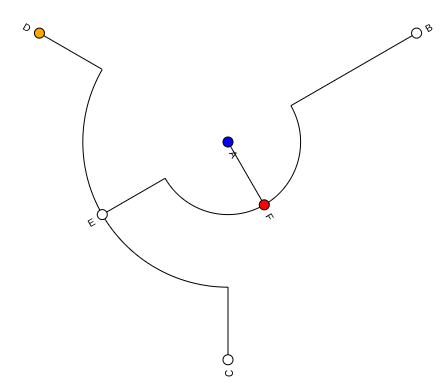
\includegraphics[width=0.7\linewidth]{imgs/phylotee}
		\caption{A Sample Tree generated by the web-component}
		\label{fig:phylotee}
	\end{figure}
	
	
	\section{Introduction}
	\subsection{What is LIS?}
	The Legume Information System is a public project funded and developed by USDA and NCGR respectively that collects and maintains genetic and genomic data of legume species. The project is used by plant biology researchers to model legumes and improve crop yields.
	\subsection{What is a Phylotree?}
	A Phylotree is a diagram designed to show the evolution of a biological species in relation to other species with similar characteristics. (See Figure 1)
	\subsection{The Project}
	LIS has been around for almost 20 years, thus, the website has gone through many iterations as technologies have advanced. So during this iteration, the project decided to implement web components into the project to improve the reusability of some functions that interact with LIS. My job was creating a web component that would visualize a Phylotree.
	\section{Preparing}
	Before the internship started, Alan assigned me a couple of resources to look into to get familiar with the Legume Information System web-component codebase. I explored TypeScript, an extended version of JavaScript, for web development, and Lit, a library designed specifically for designing web components. I also learned the Git version control system.
	\section{The Process}
    Through this project, I first looked at a previous web component that is used by LIS and was able to import some of the dependencies based on what was used in that component. The JavaScript library that was used to actually draw the tree is called TnT Tree and I used some of its documentation to structure the TypeScript type that the Phylotree would use to draw from an object. The advantage to doing this is that using the Phylotree type allows the user to include more details about the tree. For example, in the Figures 2 and 3, you can see that the nodes  have been colored by species. This is possible because of the Phylotree type. In addition to drawing the phylotree from an object, TnT can also draw the Phylotree from a text tree format called Newick, although this format doesn't contain the detailed information the Phylotree type has, it is better for use when the data the user is using is already in Newick format. This gives the web component adaptability to display using different formats as required. The web component also had additional inputs/parameters that could be set such as the ability to display in a radial or vertical format. This can be good to display the tree in a specific form. The component also had the ability to display the tree in a scaled format based on the length data provided in the input. 
    \section{Pulling data from LIS}
    LIS uses an API language called GraphQL to retrieve data. One of the data values that are stored within the GeneFamilies category is the Newick value for the tree that it contains. The LIS has already been using GraphQL for most of its web applications, so the necessary scripts were already in place to pull data into the web component. This makes it very easy to input a full tree of a GeneFamily from LIS into a Phylotree powered by our web component.
   
   
    \section{Conclusion}
    The results of this project can be seen in Figure 2 and Figure 3 as well as in the public GitHub repository. Overall, the project turned out pretty well and we were able to successfully finish the web component.  The component has been merged into a branch of the LIS web-components repository and will be moved to the main branch after some documentation and other necessary features have been added.
      \begin{figure}
        \centering
        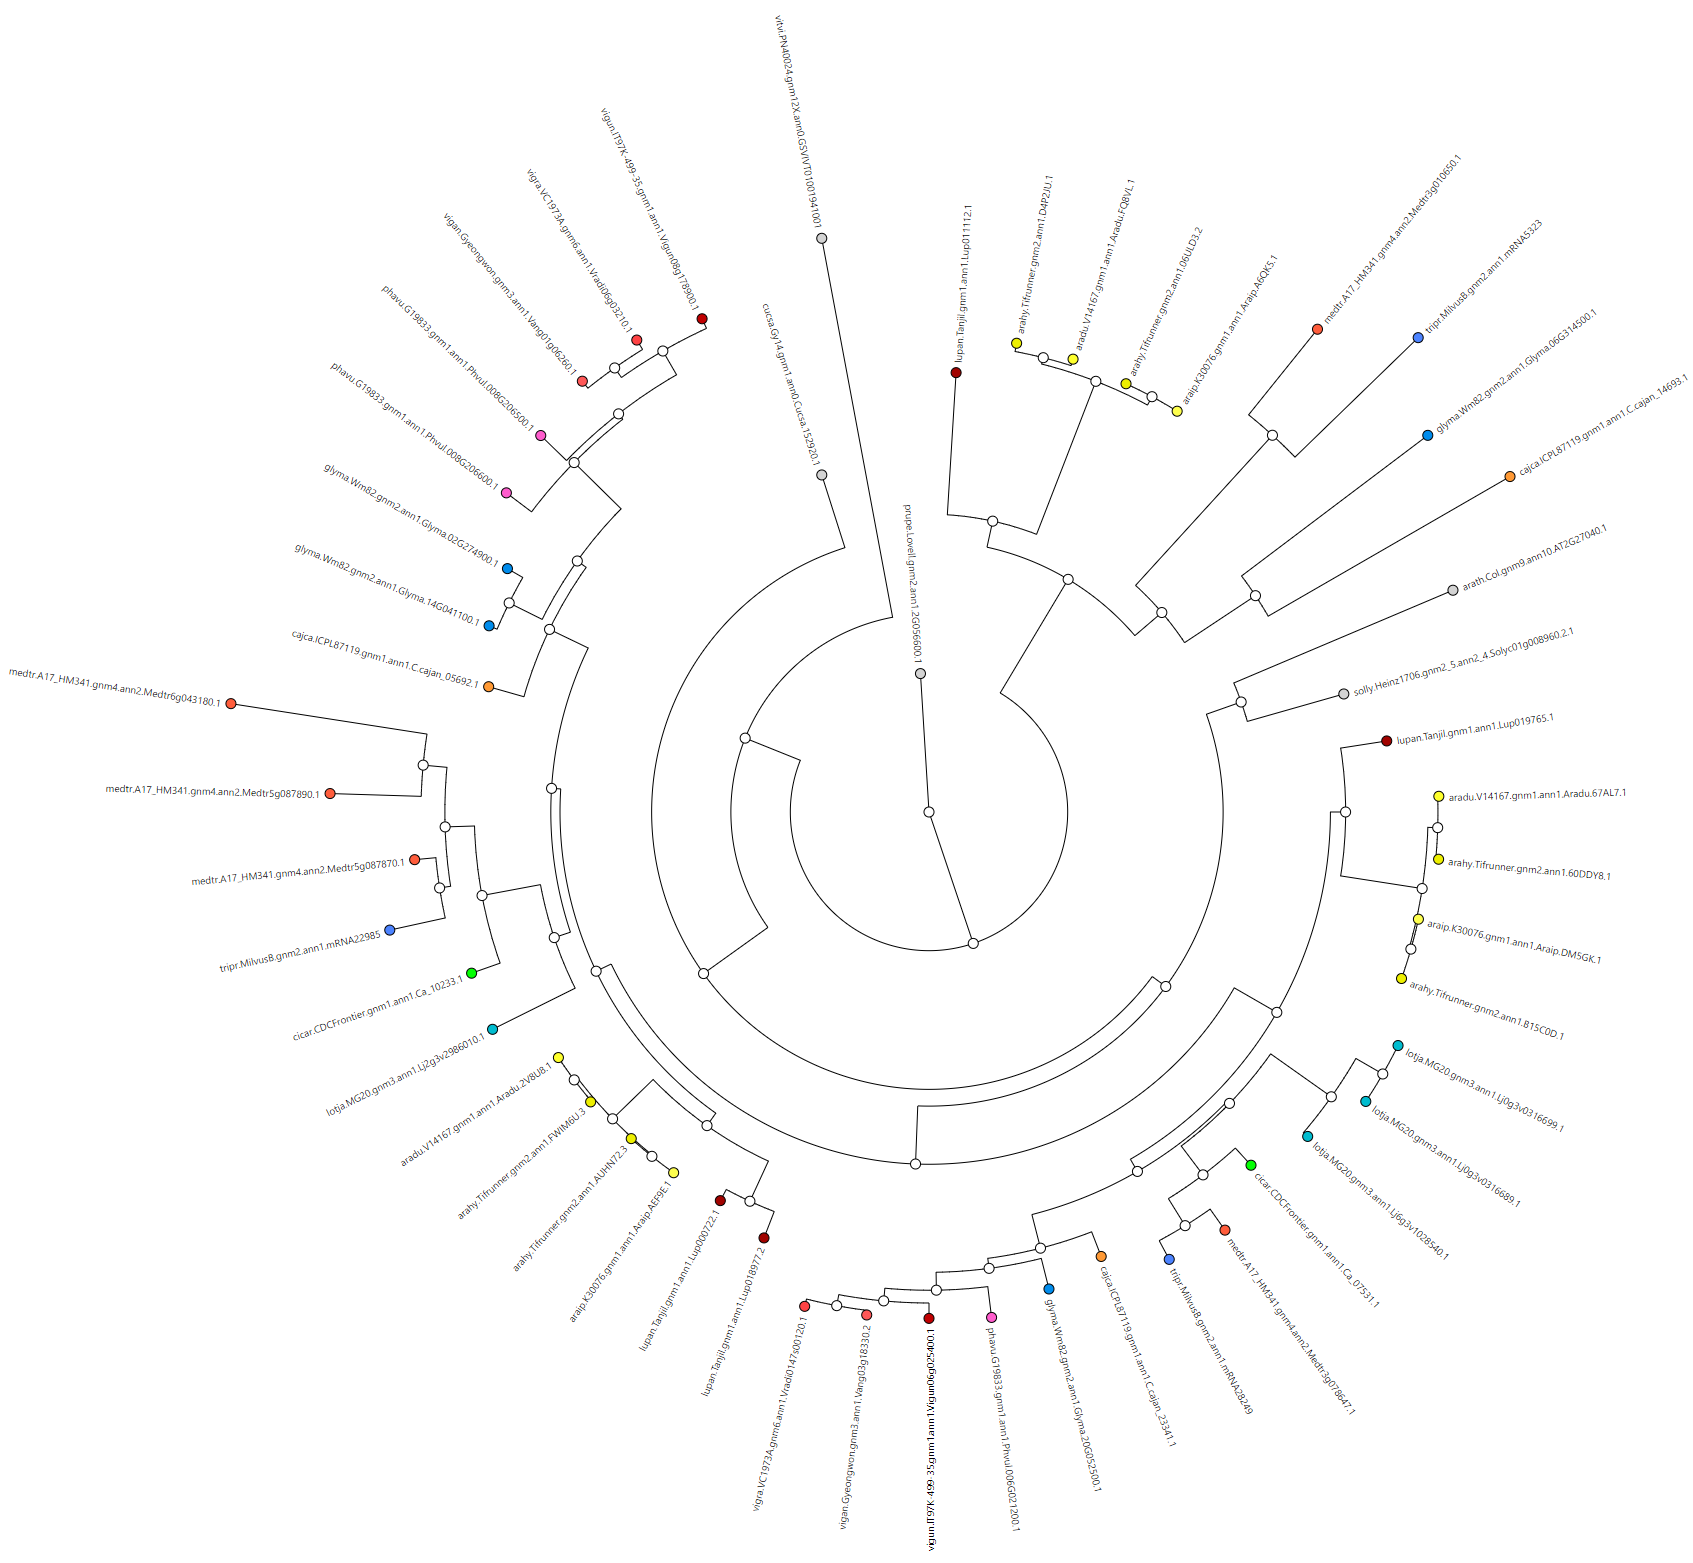
\includegraphics[width=1\linewidth]{imgs/radial-color.png}
        \caption{A radial Phylotree generated using Newick data from LIS}
    \end{figure}
     \begin{figure}
        \centering
        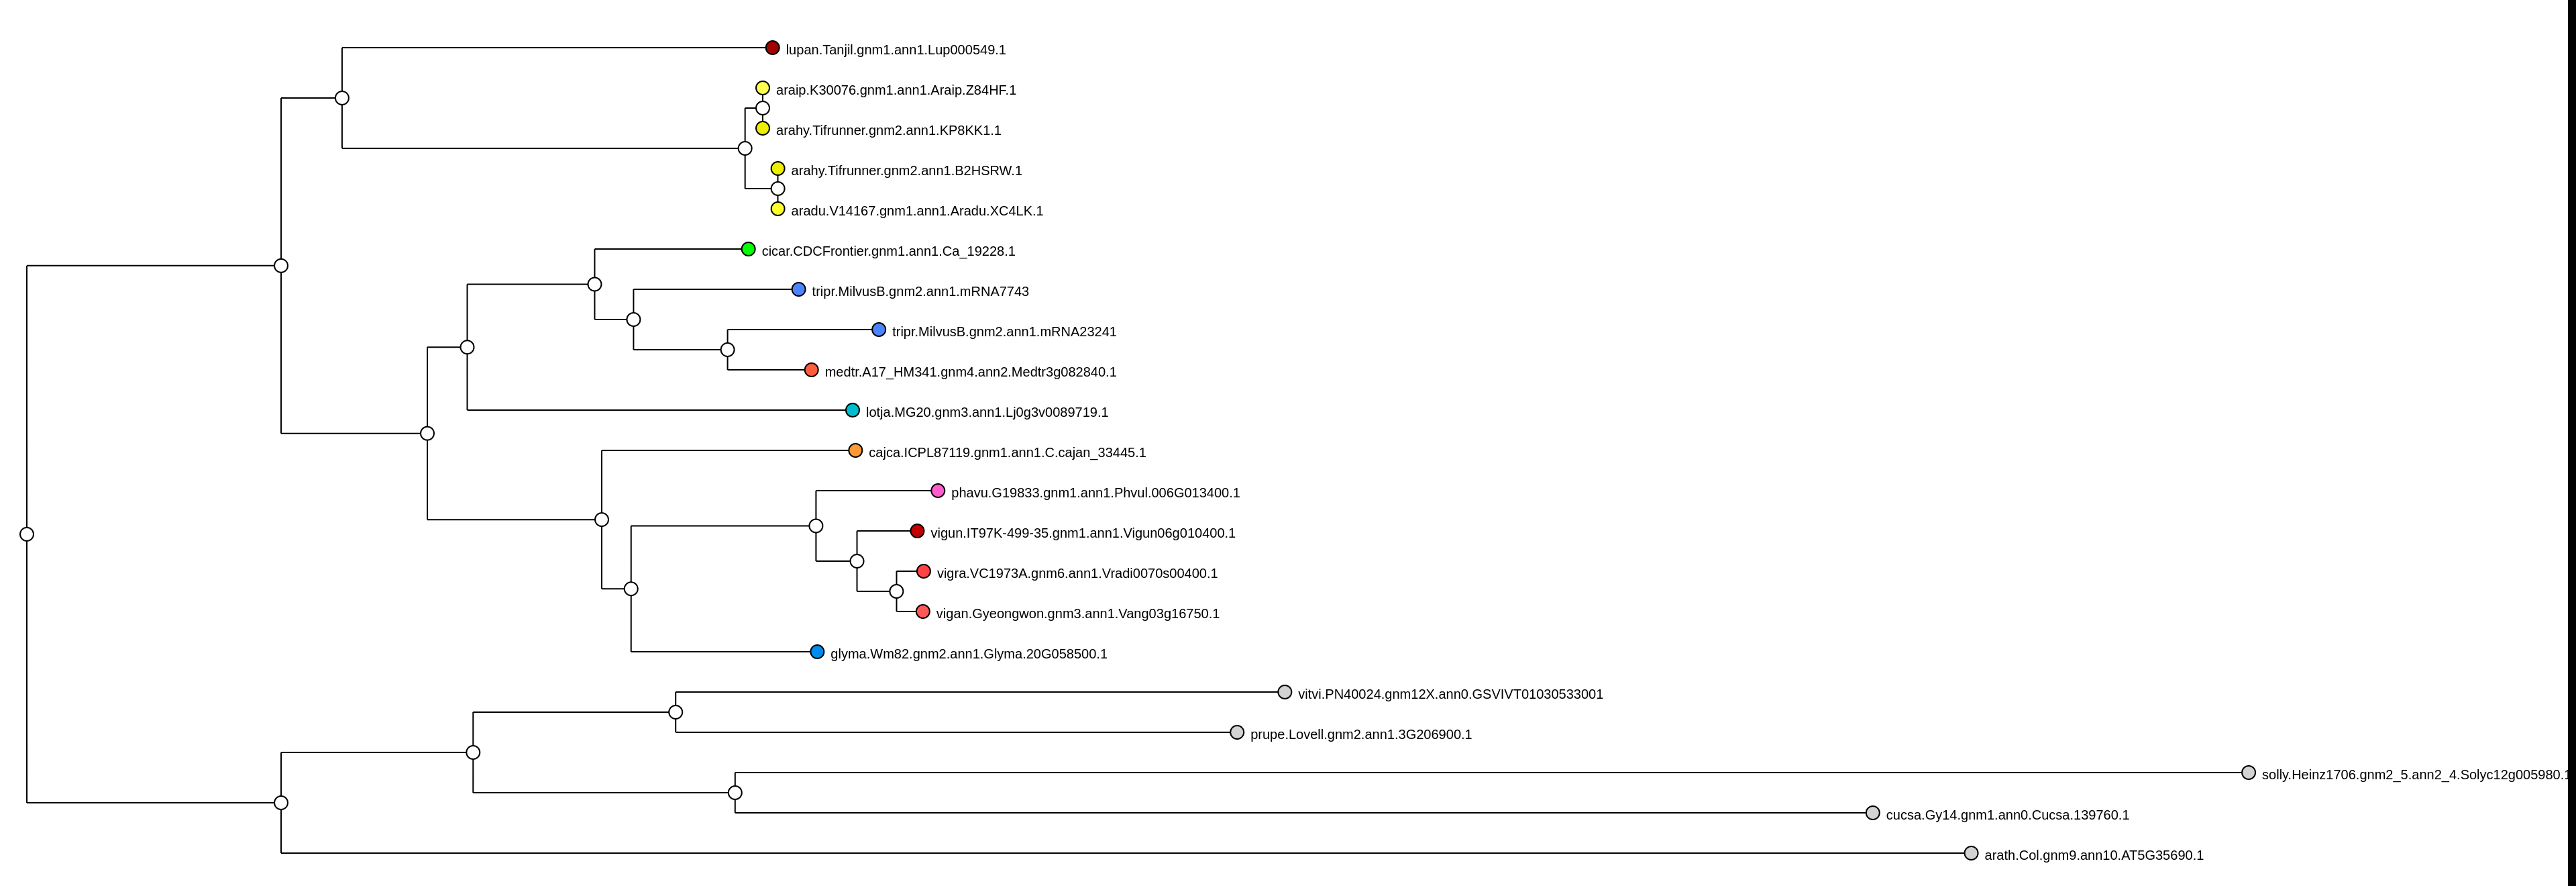
\includegraphics[width=1\linewidth]{imgs/vertical-lis-tree.png}
        \caption{A vertical Phylotree generated using Newick data from LIS}
    \end{figure}
\end{document}